\raggedright
\mychapter{3}{Work Project 3}
	\label{ch:cc}
	\section{Esercizio 1: Logica Proposizionale}
		\label{sec:es1}
		La logica proposizionale è un linguaggio formale utilizzato dagli agenti logici per la rappresentazione della conoscenza. Un agente intelligente che sfrutta tale approccio si ispira al processo umano di deduzione a partire da avvenimenti noti che ha precedentemente appreso. Quindi l'agente avrà bisogno di una base di conoscenza (\texttt{KB: knowledge base}), in cui archiviare le informazioni utilizzate nella deduzione, e di un meccanismo di inferenza (\texttt{inference engine}) per effettuare le deduzioni.
		\par
		L'agente basato sulla conoscenza, ogni volta che innesca il processo deduttivo, enuncia alla base di conoscenza la percezione corrente, dopodiché chiede ad essa l'azione da eseguire; la scelta avverrà in base alle informazioni archiviate. Comunica infine di aver eseguito l'operazione, così da garantire che l'evento scatenante il processo di ragionamento possa ampliare la propria base di conoscenza. Inizialmente l'agente può non essere a conoscenza di tutto ciò di cui necessita per completare la sua operazione, quindi sarà necessario una fase di raccolta delle informazioni iniziali. Possiamo fornire questa conoscenza al nostro agente in due modi: mediante un approccio dichiarativo vi è proprio una fase di raccolta di informazioni da parte dell'agente; nel caso di un approccio procedurale possiamo fornire noi una conoscenza iniziale all'agente. Solitamente i due approcci vengono usati insieme in modo tale da avere una buona base di conoscenza.
		\par
		
		Le informazioni non possono essere salvate nella base di conoscenza dell'agente in un linguaggio naturale, o comunque in un qualsiasi modo da cui non sia possibile trarne delle conclusioni. Per tale motivo le frasi, o formule, che costituiscono il KB, sono espresse in un linguaggio formale di rappresentazione della conoscenza. Esso determina per le formule una sintassi per esprimerle in maniera corretta ed una semantica che ne definisce la verità rispetto ad ogni mondo possibile.\par
		I mondi possibili sono gli ambienti, le condizioni in cui l'agente potrebbe venirsi a trovare. Mondi strutturati formalmente, rispetto ai quali è possibile valutare la verità delle frasi, sono più propriamente detti \emph{modelli}. Diciamo che $m$ è un modello di una frase $\alpha$ se $\alpha$ è vera in $m$. Indichiamo, inoltre, come $M(\alpha)$ l'insieme di tutti i modelli di $\alpha$.\par
		La stessa identica frase in linguaggio naturale può essere tradotta in modi differenti in base alla diversa sintassi della logica utilizzata. I concetti fondamentali del ragionamento logico sono, però, indipendenti dalla forma particolare di logica. Determinata la base di conoscenza, da essa si possono riuscire a dedurre ulteriori informazioni attraverso la relazione di \emph{conseguenza logica} (\texttt{entailment}):
		\begin{equation}
		KB\vDash\alpha \iff \alpha \mbox{ è vero in tutti i mondi in cui } KB \mbox{ è vero}
		\end{equation}
		ovvero
		\begin{equation}
		KB\vDash\alpha \iff M(KB)\subseteq M(\alpha)
		\end{equation}\par
		La conseguenza logica può essere applicata per derivare conclusioni, ovvero per eseguire \emph{inferenze logiche}. Con la notazione $KB\vdash_{i}\alpha$ si intende che $\alpha$ è derivato da $KB$ attraverso l'algoritmo di inferenza $i$. Una procedura di inferenza si dice corretta (\texttt{soundness}) se deriva solo formule che sono conseguenze logiche ($KB\vdash_{i}\alpha\Longrightarrow KB\vDash\alpha$), completa (\texttt{completeness}) se può derivare ogni formula che è conseguenza logica ($KB\vDash\alpha\Longrightarrow KB\vdash_{i}\alpha$).\par
		La logica proposizionale è una logica semplice in cui la sintassi è composta da frasi atomiche, o simboli proposizionali, legate tra loro tramite connettivi logici per ottenere formule più complesse. Un simbolo proposizionale può assumere il valore vero o falso e le regole per determinare il valore di verità di una formula, rispetto ad un particolare modello, sono definite dalla semantica: 
		\begin{itemize}
			\item $\neg P$ è vero se e solo se $P$ è falso
			\item $P\wedge Q$ è vero se e solo se $P$ e $Q$ sono entrambi veri
			\item $P\vee Q$ è vero se e solo se $P$ o $Q$ è vero
			\item $P\Rightarrow Q$ è falso se e solo se $P$ è vero e $Q$ è falso
			\item $P\Leftrightarrow Q$ è vero se e solo se $P$ e $Q$ sono entrambi veri o entrambi falsi
		\end{itemize}
		%la negazione che muta il valore della nostro letterale, l' operazione di and che ci da vero solo se i due connettivi sono veri, or restituisce vero se uno dei due è vero, implicazione ci dà falso se dal vero deduciamo il falso e quella bicondizionale vera se e solo se entrambi i letterali hanno lo stesso significato.
		Queste regole possono anche essere espresse con le \emph{tabelle di verità}, che esprimono i valori di verità di una frase complessa per ogni possibile configurazione dei suoi simboli proposizionali.\par
		Come procedura di inferenza possiamo ricorrere ad un approccio per enumerazione (\texttt{model checking}): enunciamo tutti i possibili modelli, tramite la tabella di verità, e verifichiamo che $\alpha$ sia vera in ogni modello in cui KB è vera. I modelli sono rappresentati da un assegnamento di valori vero o falso ad ogni simbolo proposizionale. Questo algoritmo è corretto e completo, ma è molto oneroso in quanto i possibili mondi sono tanti (crescono esponenzialmente) ed enumerarli tutti comporterebbe una notevole complessità spaziale e temporale.
		\par
		Per tale ragione si preferiscono altri approcci basati sull'applicazione delle regole inferenziali. Esaminiamo l'algoritmo di risoluzione, strettamente legato al concetto di \emph{soddisfacibilità}. Una frase è soddisfacibile se è vera in qualche modello, viceversa insoddisfacibile se non è vera in nessun modello. La soddisfacibilità è connessa all'inferenza dalla:
		\begin{equation}
		KB\vDash\alpha \iff KB\wedge \neg \alpha \mbox{ è insoddisfacibile}
		\end{equation}
		La procedura inferenziale tenterà, dunque, di provare $\alpha$ attraverso una \emph{reductio ad absurdum}, ovvero dimostrando che $KB\wedge \neg \alpha$ è falsa in ogni modello. 
		Prima di tutto dobbiamo trasformare le frasi complesse nella forma \emph{CNF} (\texttt{Conjunctive Normal Form}), cioè come congiunzioni di clausole (disgiunzioni di letterali), attraverso le regole di equivalenza logica. %purtroppo anche qui c'è un grande sforzo dell' essere umano che deve applicare tali regole affinché sia possibile dedurre qualcosa.
		Si cerca, poi, di dimostrare che la congiunzione della base di conoscenza con il negato della frase da dedurre sia insoddisfacibile, cioè non esista nessun modello in cui $KB$ non implichi $\alpha$. Se ciò fosse provato, significherebbe che in tutti i mondi in cui è vera la base di conoscenza, sarebbe vera anche la frase. Si considerano, allora, coppie di clausole della frase complessa $KB\wedge \neg \alpha$ alle quali si applica la regola di risoluzione inferenziale: si produce una nuova clausola che contiene tutti i loro letterali tranne quelli complementari ($l$ e $\neg l$). Si provvede ad 
		applicare questo ragionamento ricorsivamente fino a che non si riescono più a generare nuove clausole, ottenendo esito negativo, oppure si arriva alla clausola vuota, rappresentante la deducibilità della frase dalla base di conoscenza. Anche questo algoritmo è corretto e completo per la logica proposizionale.\par
		In ogni caso l'agente non conosce il significato della frase, che le può essere attribuito, invece, dall'essere umano: l'agente è solo capace di applicare le regole inferenziali.
		
		%Le informazioni non possono essere salvate nella base di conoscenza dell'agente in un linguaggio naturale, o comunque in un qualsiasi modo da cui non sia possibile trarre delle conclusioni. Per tale motivo le frasi, o formule, che costituiscono il KB, sono espresse in un linguaggio formale di rappresentazione della conoscenza. Esso prevede una sintassi, per esprimerle in maniera corretta, ed una semantica, che gli attribuisce un significato. %possiamo vedere la semantica come un legame tra il mondo reale e quello della rappresentazione.
		%che ne definisce la verità rispetto ad ogni mondo possibile%.
		%La stessa identica frase espressa naturalmente può essere tradotto in modi differenti in base alla diversa sintassi della logica che andiamo ad utilizzare. Infatti il risultato da ottenere, determinare se delle evidenze possono implicare dei fatti (\texttt{entailment}) è indipendente dalla logica utilizzata per la traduzione.
		% cioè avendo dei dati noti a priori, capire se si può riuscire a dedurre altre informazioni che a noi interessa sapere, tale relazione è detta di implicazione(entailment).
		%Utilizzeremo la logica proposizionale, in cui la sintassi è composta da frasi atomiche, legate tra loro tramite connettivi logici per ottenere frasi più complesse, il singolo elemento della frase può assumere valore vero o falso,infatti la semantica di tale logica è quella di trovare i mondi in cui la frase risulta vera. Le operazioni tra i letterali sono: la \textbf{negazione} che muta il valore della nostro letterale; l' operazione di \textbf{and} che ci da vero solo se i due connettivi sono veri;l'operazione di \textbf{or} restituisce vero se uno dei due è vero;l' \textbf{implicazione} ci restituisce falso se dal vero deduciamo il falso e infine quella \textbf{bicondizionale} vera se e solo se entrambi i letterali hanno lo stesso significato.
		%Per verificare la relazione di implicazione possiamo ricorrere a due strade, la prima è quella in cui enunciamo tutti i possibili mondi del nostro modello, per esempio tramite la tabella di verità, tra questi individuiamo quelli che rendono veri la nostra base di conoscenza e la deduzione che stiamo facendo e se i mondi che rispecchiano la nostra percezione sono contenuti all' interno del concetto che vogliamo dedurre, allora possiamo dire che la nostra conoscenza implica quel fatto.
		%Sulla tabella possiamo vederlo facilmente basta verificare che per ogni riga in cui la nostra evidenza è vera anche la frase che vogliamo implicare lo sia.
		%\par
		%Tale metodo è molto oneroso quando i possibili mondi sono tanti, enumerarli tutti sarebbe molto dispendioso sia in termini di spazio che di tempo, per tale ragione di preferiscono altre strade.
		%\par
		%Una possibile è scrivere le frasi in forma CNF e da li applicare metodi inferenziali per capire se la nostra conoscenza implica il fatto. 
		%Prima di tutto però dobbiamo trasformare le frasi che abbiamo nella forma CNF, cioè or di congiunzioni atomiche, per farlo sfruttiamo le regole di equivalenza logica. Purtroppo anche con questo metodo c'è un grande sforzo dell' essere umano che deve applicare tali regole affinché sia possibile dedurre qualcosa.
		%Quando la conoscenza, è nella forma da noi voluta, possiamo provare a dimostrare che questa, renda non soddisfacibile il negato della frase che vogliamo dedurre, cioè non esista nessun modello che implica quella frase. Se ciò accade significa che la frase non negata è valida, cioè in tutti i mondi in cui è vera la nostra base di conoscenza anche la frase lo è. Per verificare che not A sia insoddisfacibile, basta prendere una coppia di clausole(congiunzione di letterali), presenti nella nostra base di conoscenza ed iniziare a derivare nuove informazioni, ciò avviene quando nella frase che si viene a creare si presentano due letterali complementari (A e not A).
		%Applichiamo questo ragionamento ricorsivamente fino a quando non riusciamo più a determinare nuove clausole e quindi quel fatto non è deducibile dalla nostra conoscenza, oppure si arriva alla clausola nulla, potendo affermare che la not A non è soddisfacibile.
		%Tali situazioni implicano la validità della clausola di partenza A.
		%\par
		%Tutti e due algoritmi sono completi e soundness.
		%Un algoritmo è completo se é capace di enumerare tutte le relazioni di implicazione possibili dalla base di conoscenza.
		%Un algoritmo è soundness quando ogni implicazione dello stesso, rispecchia quelle della base di conoscenza.
		%Per entrambe le procedure enunciate vale il discorso che l' agente non conosce il significato della frase, quello è dato dall' essere umano, per l' agente una frase vale un' altra, esso è solo capace di applicare le regole inferenziali, non riuscendone infatti a discernere il significato.
		
		\section{Esercizio 2: Reti Bayesiane}
		\label{sec:es2}
		L'approccio probabilistico, rispetto alle altre tipologie, tiene conto del grado di incertezza. Infatti, a differenza di un approccio logico in cui un fatto può essere vero o falso, nell'approccio probabilistico si considera la probabilità dell'avvenimento. Tale livello d'incertezza non ci assicura a priori la verità di un'affermazione: affermando che oggi pioverà con una probabilità di 0.99, potrebbe capitare che non piova, proprio perché la probabilità definisce il livello di incertezza rispetto ad una conoscenza da noi acquisita che varia da persona a persona (agente ad agente), dipendente da esperienze diverse che determinano valori di incertezza diversi. Le reti Bayesiane si rifanno al concetto di probabilità, più propriamente alla regola di Bayes così definita:
		\begin{equation}
			P(causa|effetto)=\frac{P(effetto|causa)*P(causa)}{P(effetto)}
		\end{equation}
		Una rete Bayesiana di solito è fatta in questo modo:
		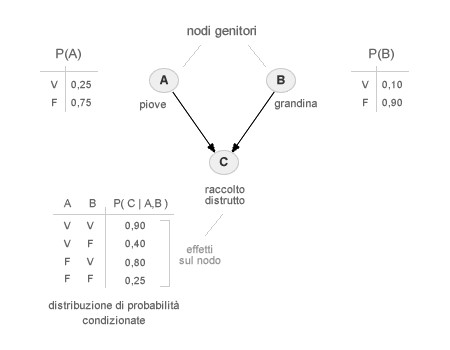
\includegraphics[width=0.95\textwidth, height=0.40\textheight]{retebayesiana.jpg}
		Come possiamo osservare, ci sono dei nodi che determinano la variabile aleatoria da tenere in considerazione, a cui si assegnano anche i relativi valori di probabilità a priori, e dei collegamenti che indicano la relazione di causalità tra i nodi, rappresentati dagli archi orientati.
		\par 
		Per realizzare tale rete dobbiamo tenere conto delle relazioni di causalità delle nostre variabili, così facendo otteniamo una rete che riesce ad esplicare bene le nostre conoscenze. Una peculiarità di questa rete è la compattezza, infatti qualsiasi altro modo di realizzare la rete ne aumenterebbe la complessità. Una rete così realizzata permette di effettuare calcolo delle probabilità in modo semplice, perché  in una rete siffatta vale l' indipendenza condizionata: una volta definito un valore per una variabile padre, le variabili figlie sono indipendenti tra di loro. Per esempio, se la variabile A è padre di B e C, la probabilità $P(B\wedge C|A)=P(B|A)*P(C|A)$; se non avessimo l'indipendenza, non potremmo scrivere i due domini separati e dovremmo tener conto anche della probabilità di B dato C. Per queste reti si definisce anche il concetto di semantica locale, cioè ogni nodo è indipendente dai suoi non discendenti dato il nodo padre, e della coperta di Markov, ovvero un nodo è indipendente da tutti gli altri dato il nodo padre, i figli e i padri dei figli.
		\par  
		Per ricavare dati da queste reti, date le probabilità a priori, possiamo semplicemente calcolare tutti i valori di probabilità a posteriori che ci occorrono, metodo complesso nel caso in cui la rete sia grande e il numero di possibili valori delle variabili sia elevato. Di solito si può ricorrere all' approccio frequentista, che consiste nel generare un token che avrà una probabilità di ottenere un valore del nodo pari proprio all' incertezza legata ad esso, dopodiché si inizia a campionare la rete facendo scorrere il token su di essa, fissandone i valori con quelli risultanti dal campionamento. Le configurazioni ricavate, una volta raggiunta la quantità di risultati voluti, vengono divise per il numero dei campioni valutati, tenendo conto della loro molteplicità. Tale metodo per un alto numero di eventi determinati deve tendere all' approccio di calcolare le probabilità a posteriori. Le reti bayesiane così costruite sono statiche perché non tengono conto di un riferimento temporale. Le reti bayesiane dinamiche tengono conto anche di un valore temporale, suddiviso in istanti. In questo caso la variabile casuale non avrà solo relazioni con altre variabili, ma anche con se stessa valutata in istanti diversi di tempo. I valori di probabilità che di solito vengono ricavati su tali reti sono: il \texttt{filtering}, cioè la probabilità che avvenga un determinato evento all' istante t dati gli eventi precedenti e l' evidenza; lo \texttt{smoothing}, la probabilità di un evento in un istante t-k, con k che va da 0 a t, data l'evidenza fino all'istante t, utilizzato per correggere la probabilità relativa ad un fatto da un istante ad un altro;
		la \texttt{previsione}, la probabilità di un evento all' istante t+k, con k>1, dati gli eventi e l'evidenza fino a t;
		la \texttt{spiegazione migliore}, la sequenza di stati che più probabilmente ha generato l'evidenza data.
		\par 
		Il \texttt{filtering} può essere facilmente calcolato ricorsivamente. Conoscendo il fatto iniziale ed essendo i processi stazionari, possiamo determinare il risultato del filtraggio all'istante precedente e calcolare il risultato grazie alla nuova evidenza.
		%quello all' istante successivo e poi pesare la probabilità dello stato data l' evidenza.
		Questo è possibile per la stazionarietà dei processi, cioè i cambiamenti sono regolati da leggi immutabili nel tempo, ovvero la tabella di probabilità di un fatto non cambia rendendo tale relazione identica ad ogni avanzamento.
		Esiste anche una tecnica detta di \texttt{particle filtering}, che prevede un campionamento sul fatto iniziale, la propagazione di tali esempi sul campione successivo, la pesatura in base all'evidenza ed il ricampionamento per lo stato successivo, tenendo conto del nuovo peso dei campioni. Ovviamente per ottenere il valore di probabilità di una determinata configurazione dobbiamo dividere il numero di casi uguali per il totale di campionamenti effettuati, e per un alto valore di quest'ultimi la probabilità tenderà a quella reale che avremmo ottenuto con il filtering. Tali reti possono essere usate anche nel machine learning. Dato un insieme di ipotesi, possiamo vedere qual è la probabilità associata ad esse data un'evidenza, cioè calcolare la probabilità di $P(hi|d)$ dove hi è l'ipotesi e d l'evidenza. Siamo interessanti alla probabilità di ogni ipotesi (sommatoria). Ad ogni nuova evidenza potrebbe variare la hi che massimizza la probabilità. Non è molto agevole portare avanti i calcoli per tutte le ipotesi, per tale ragione si sceglie quella che massimizza il valore a posteriori (\texttt{MAP}), cioè l'ipotesi che massimizza $\alpha*P(d|hi)*P(hi)$, dove $\alpha$ è la costante di normalizzazione. Nel caso in cui le ipotesi abbiano probabilità a priori uguali (stessa complessità), si può usare la \texttt{maximum-likelihood (ML)}, che consiste nel massimizzare $P(d|hi)$.
		Potremmo pensare all'uso dei logaritmi nel caso in cui compaiano esponenziali rendendo la massimizzazione della derivata molto più semplice.
		
		\section{Esercizio 3: Reti Neurali}
			\label{sec: es3}
			Le reti neurali sono un meccanismo computazionale che si ispira al funzionamento del cervello umano. Sono rappresentabili tramite un grafo orientato, i cui nodi costituiscono un modello matematico del neurone, e agli archi orientati è associato un peso. Ogni nodo \textit{i} calcola la sua uscita $a_{i}$ applicando una funzione di attivazione \textit{g}, chiamata \texttt{activation function}, alla somma pesata degli ingressi.% propagatisi dai nodi \textit{j} tramite l'arco corrispondente di peso $W_{i,j}$.
			\begin{equation}
			a_{i} = g(in_{i}) =g( \sum_{j=0}^n W_{j,i} a_{j})
			\end{equation}
			\medskip
			\begin{center}
				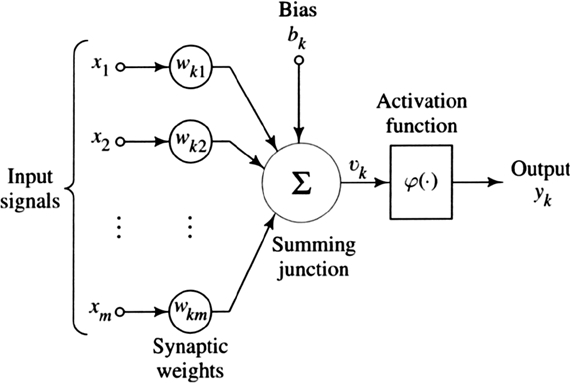
\includegraphics[width=0.8\textwidth, height=0.3\textheight]{neurone.jpg}
			\end{center}
			La funzione di attivazione storicamente utilizzata era quella di \emph{soglia}; in seguito si è diffusa la funzione \emph{sigmoide}, continua e derivabile rispetto alla precedente.\par
			Possiamo classificare strutturalmente le reti neurali distinguendo le \texttt{Recurrent Networks} e le \texttt{Feed-Forward Networks}. Le ultime non si fondano sul concetto di stato interno, a differenza delle prime. Inoltre possono essere suddivise in più livelli, o \emph{layers}. Le reti neurali a singolo layer riescono a rappresentare solo operazioni \emph{linearmente separabili}, a due layer tutte le funzioni continue, a tre layer anche le funzioni discontinue.
			\begin{center}
				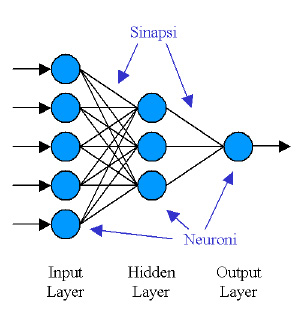
\includegraphics[scale=0.6]{RN-multilayer.jpg}
			\end{center}
			\par
			Una difficoltà non trascurabile risiede nella costruzione della struttura della rete neurale. Esse, infatti, sono sistemi \texttt{black-box}, il cui funzionamento interno è di difficile interpretazione logica, anche se è possibile averne una matematica che non aiuta nella sua costruzione.
			\par
			Per determinare il peso degli archi si utilizza l'algoritmo di \texttt{Back-Propagation}. Inizialmente si costituisce una rete con pesi casuali o uniformi per abolire l'onere computazionale. Consideriamo poi una coppia ingressi-uscita del data-set. L'errore tra l'uscita ottenuta e quella desiderata verrà propagato all'indietro per ogni  livello, così da modificare i pesi ed ottenere una migliore approssimazione della funzione. Tale propagazione fa uso del \texttt{learning rate} per far si che un singolo esempio non influisca interamente sui valori dei pesi, altrimenti questi tenderebbero ad oscillare di molto nel caso in cui ogni esempio fornisca un errore relativamente grande. La procedura verrà iterata per ogni esempio, ciascuno dei quali consentirà una correzione dei pesi, delineando una struttura della rete coerente con la funzione da approssimare. I problemi principali che riscontriamo in questo algoritmo sono l'eccessiva complessità temporale e la possibilità di arresto su di un minimo locale.\par
			Per quanto riguarda, invece,la determinazione del numero di neuroni, si procede tipicamente con un approccio \texttt{trial and error}, perché non è chiaro precisamente il significato della rete. Si parte, quindi, da reti semplici: se queste dopo la \texttt{Back-Propagation} funzionano bene, le si usa, altrimenti si iniziano a inserire nuovi neuroni o layer di neuroni e si continua a testare la validità delle nuove reti create.\par
			In definitiva, le reti neurali si sono rivelate empiricamente un buon approssimatore di funzioni ed oggi il loro utilizzo ha ripreso vigore nella forma di \texttt{Deep Learning}. Tali tecniche ottengono un basso \emph{error rate} nei problemi relativi al riconoscimento di caratteri e sono largamente diffuse nei sistemi multimediali per quanto concerne il riconoscimento di immagini, audio o nella \texttt{Computer Vision} in generale. Seppur presentando buoni risultati, bisogna ricordare che \emph{non esiste un algoritmo di apprendimento migliore in assoluto, ma bisogna trovare quello più adatto al problema dato.}
			
		\section{Esercizio 4: Cloud e Crowdsourcing}
			\label{sec:es4}
			Il \texttt{Cloud Computing} ed il \texttt{Crowdsourcing} sono paradigmi affermatisi nel nuovo millennio, figli della dirompente rivoluzione della rete non solo al livello culturale, ma anche economico, fornendo nuovi modelli per sviluppare ed offrire servizi al cliente.\par
			Il cloud prevede l'erogazione di risorse informatiche \emph{on demand} attraverso Internet. Tipicamente, in linea del tutto generale, un \texttt{Cloud Provider} fornisce un \emph{pool} condiviso di risorse; esse possono essere configurate da un cliente amministratore che le carica di valore aggiunto; infine l'utilizzatore finale usufruisce delle risorse in tal modo configurate per poi rilasciarle al termine del suo utilizzo.\par
			Il crowdsourcing è lo sviluppo collettivo di un progetto da parte di volontari esterni al suo ideatore. Questo fenomeno deriva dalla nascita delle prime \emph{open community} di condivisione, legate profondamente al concetto di \emph{sharing}. Le \emph{community open source} sono state le prime a sfruttare i benefici del crowdsourcing. Questo paradigma si è diffuso anche in ambito aziendale con il modello di business di \emph{open enterprise}.\par
			Quantopian applica questi concetti fornendo i servizi per scrivere algoritmi di trading e rendendoli disponibili all'intera community, nella quale si potranno condividere idee, codice e dati. Esso, inoltre, investe sugli algoritmi con le migliori performance, condividendone i profitti con l'autore. Rappresenta, dunque, un modello di business all'avanguardia, che sfrutta pienamente le potenzialità della community, guidandola tramite i propri strumenti e ricavando introiti dall'impulso creativo a cui il crowdsourcing porta.
			\par 
			Tale piattaforma offre molti dataset direttamente, evitando l'esigenza di importarli da altre fonti. Nel nostro esempio vediamo operazioni di trading su azioni americane di una nostra possibile società, che ha un certo numero di azioni iniziali e decide quando vendere o comprare tali titoli per aumentare i suoi introiti partendo da un capitale iniziale ed osservando cosa accade in un determinato lasso di tempo.
			\par 
			Il codice fornisce tale output:
			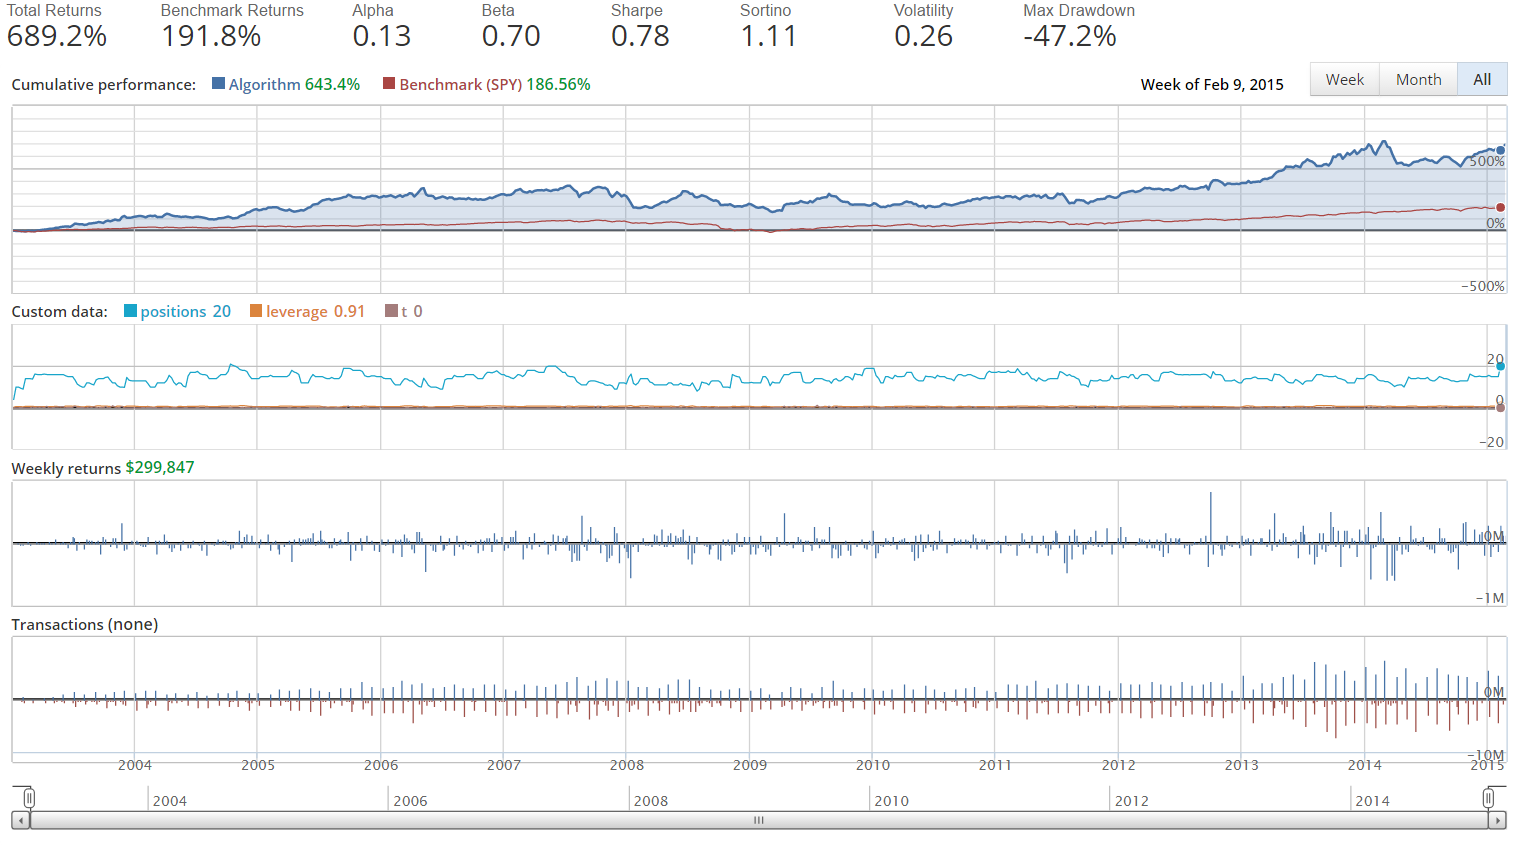
\includegraphics[width=1.0\textwidth, height=0.40\textheight]{inizio.png} 
			La linea rossa definisce il reale valore che si avrebbe avuto confrontandosi con il mercato, quella blu determina la previsione stimata dall'algoritmo, il valore position ci dice il numero di azioni attive, cioè non ancora chiuse, leverage ci dice quanto siamo disposti ad investire in base agli introiti, il guadagno settimanale è la transazione monetaria che c'è stata.
			Come si può vedere dall' esempio, le nostre scelte di trading secondo il nostro algoritmo sono molto rosee rispetto a ciò che è successo realmente, anche se a grandi linee, comunque, la previsione rispetta l'andamento avuto, dandoci però un guadagno falsato.
			La modifica dell'algoritmo, permessa a qualsiasi utente tramite cloud, viene eseguita da un \emph{server farm}, sicuramente più performante di un pc qualunque. Difatti, in figura sono rappresentate le valutazioni del mercato americano di circa 12 anni, un onere di computazione non banale. \par
			Una possibile modifica dell'algoritmo è puntare solo sulle azioni che ci danno un valore di utile maggiore:
			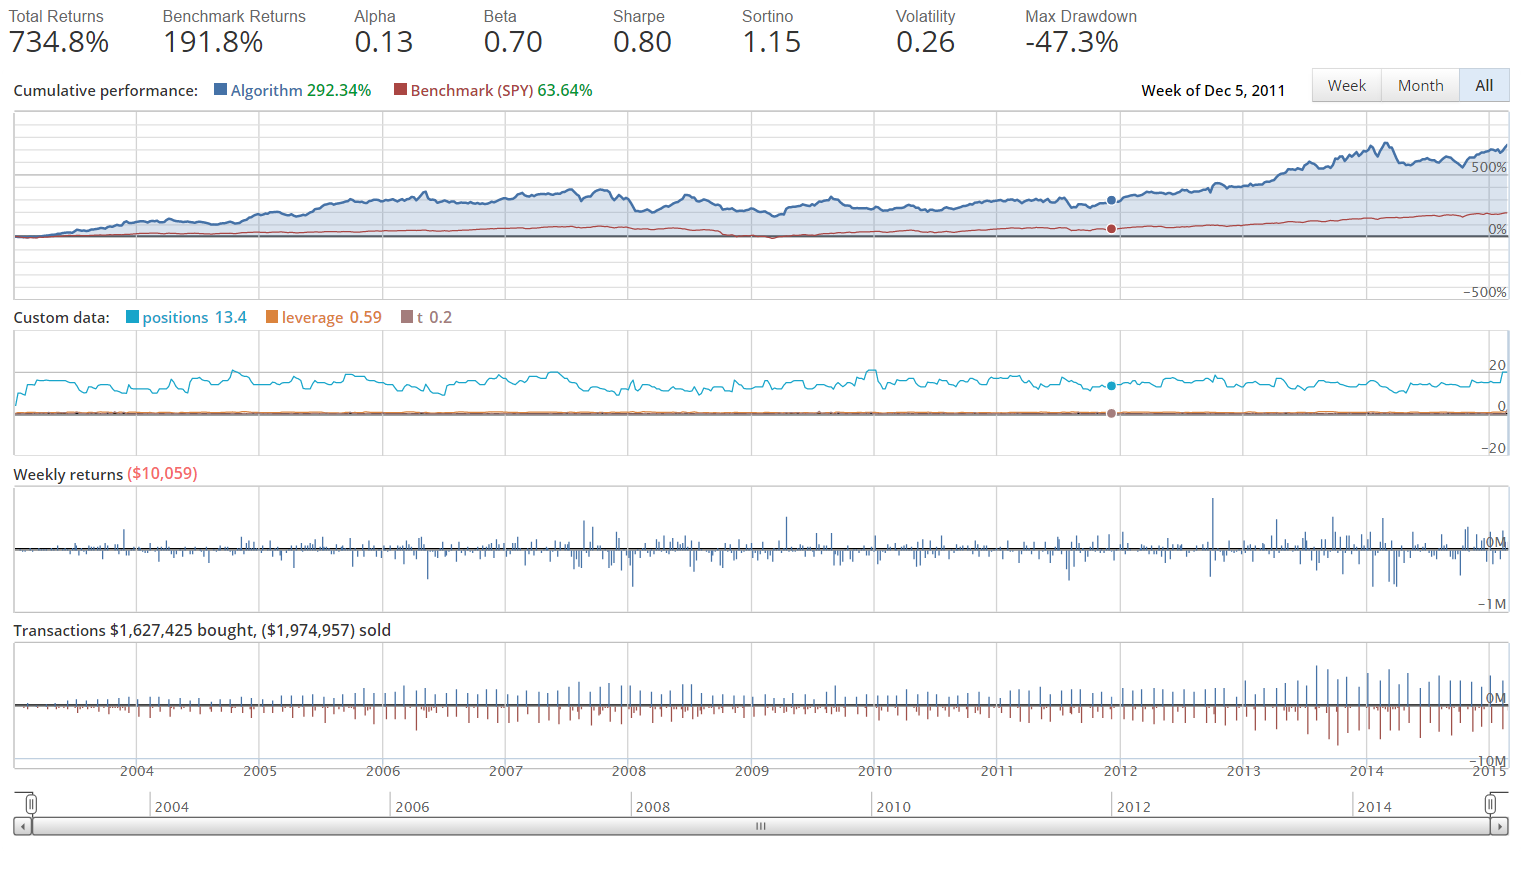
\includegraphics[width=1.0\textwidth, height=0.40\textheight]{factorfilter0,1.png} 
			Come vediamo, l'algoritmo si è comportato meglio, perché sono state prese solo le 3000 azioni che davano un'utilità sperata maggiore, quindi abbiamo fatto trading su azioni che ci permettono di massimizzare i guadagni. Questa è un operazione che di solito premia a lungo termine. Non è sempre detto, però, che un'azione abbia il comportamento sperato, perchè può capitare che la sua efficienza sia minore a causa di fattori non ancora accaduti, che potrebbero in effetti portare ad un'utilità diversa.
			Un altro esperimento è stato quello di aumentare il profitto che si voleva fare con una determinata azione, tendendo quindi a cercare di sfruttare quanto più quell'azione per massimizzare i guadagni. Il risultato è peggiorato:
			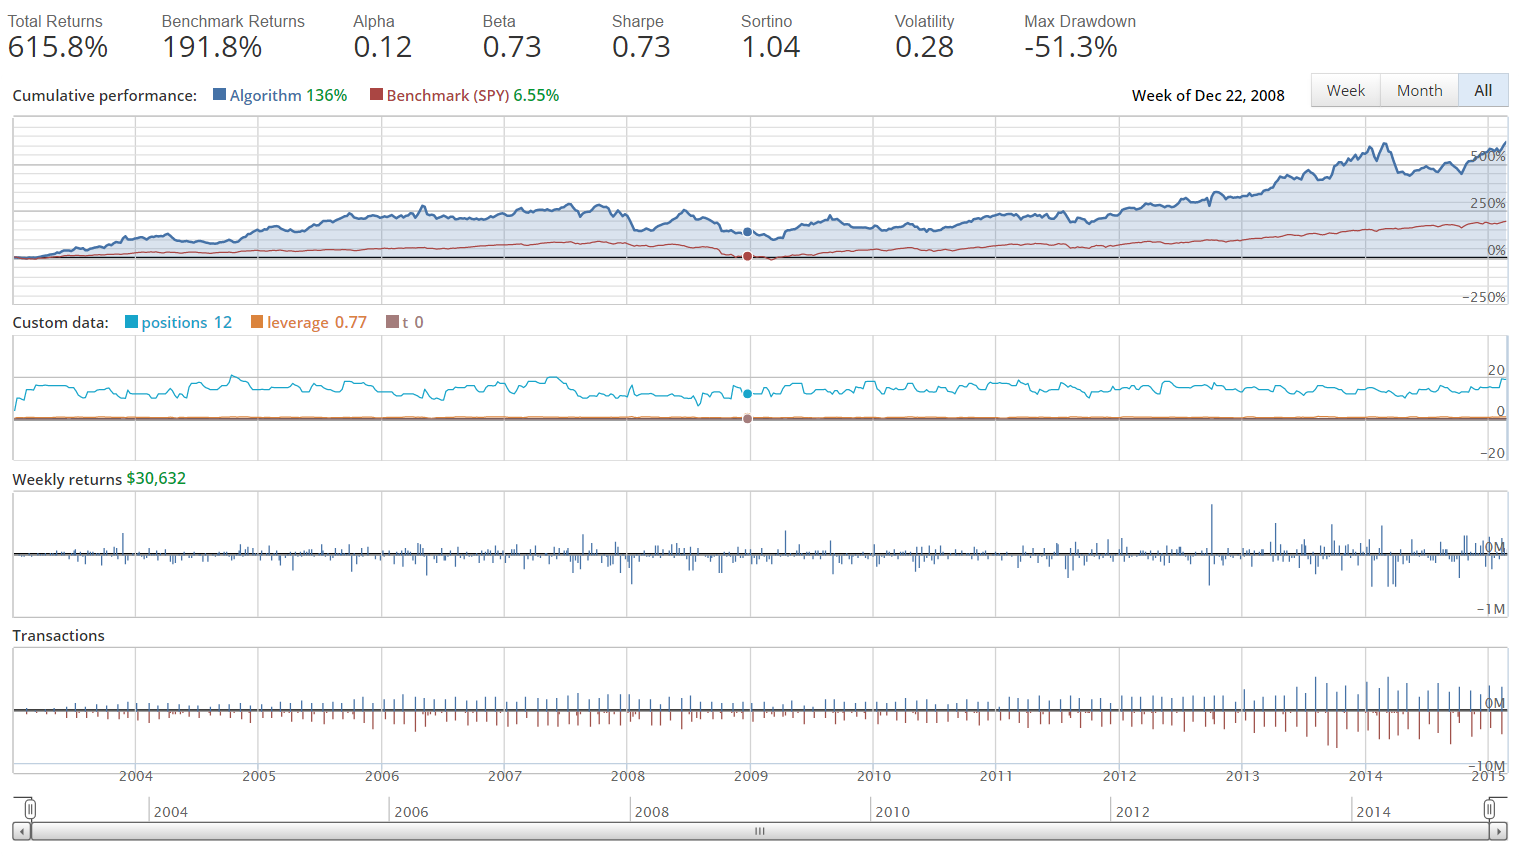
\includegraphics[width=1.0\textwidth, height=0.40\textheight]{stock2.png} 
			Possiamo vedere che il numero di transazioni è minore rispetto ai due casi precedenti, appunto perché una volta che si è iniziato a fare un trade su quell'azione, fino a che non ci porta al guadagno voluto o scende al di sotto di un valore minimo, non la vendiamo. In tal modo abbiamo cercato di attuare una politica più conservativa sulla compravendita, che ci ha portato a dei ricavi minori, ma ad un atteggiamento più consono a quello che in realtà è successo.